\chapter{付録}
実装したアプリのソースコードを掲載する。実装はswift7.0を用いて、iPhone 9.2での動作を確認している。これらソースコードパッケージの最新版はGithubの以下のURLにて公開している。 \\
https://github.com/risahiyama

\section{DreamDateプロトタイプ}
DreamDateがスマートフォンアプリで睡眠中に音を流すという形に至った背景を述べる。
\subsection{刺激提示のプロトタイピング}
人には視覚、聴覚、触覚、味覚、嗅覚を含む5つの感覚器がある。本研究ではそのうちの聴覚と嗅覚による刺激が睡眠中の夢に与える影響を実験を通して観察した。

\subsubsection{香りによる刺激}
\begin{figure}[htbp]
\begin{center}
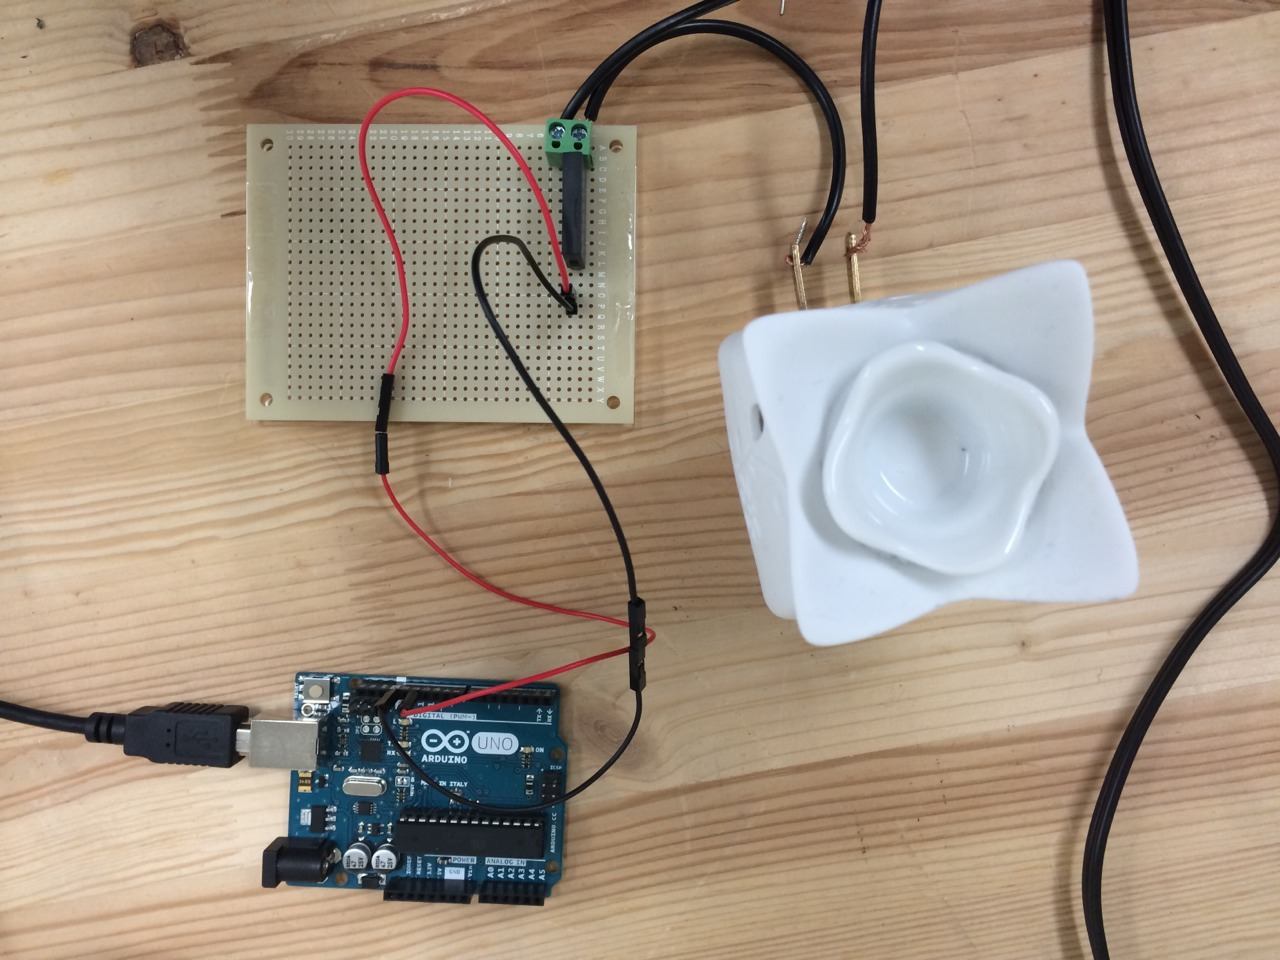
\includegraphics[width=9cm]{eps/smell.eps}
\caption{香りによる刺激}
\label{smell}
\end{center}
\end{figure}

 ラベンダーやバラのような良い香りは睡眠に良い影響を与え、心地良い夢を見やすくするということはMichael SchredlとBoris Stuckの研究によって証明されている\cite{roseDream}。しかし香りが夢の内容に影響を与えるか否かの研究はまだ行われていない。そこでこのプロトタイプはレム睡眠の時に思い出と直結する香りを出して夢を刺激することで夢になんらかの影響を与えられるものか否かを確かめるために製作した。\\
 加速度センサーでレム睡眠を検出したらアロマランプに光がつき、5分後香りが部屋中に充満するという作りになっている。図\ref{smell}にあるのはそのプロトタイプの写真である。実験に参加したのは嗅覚が正常に機能している(風邪などを引いていない)22歳の女性3名。被験者1には交際相手が部屋で使っているアロマとコーヒー豆の香りで刺激した。被験者2と被験者3はコーヒー豆の香りで刺激した。その香りをたくとすぐに過去の思い出と直感的に繋がる香りをあえて選び、アロマライトは被験者の頭のすぐ横に置いた。\\
 2015年の1月に10日間の実験を行った。香りありの夜、香りなしの夜を5日間ずつ交互に繰り返した。その結果を図\ref{smellExperiment}に示す。

\subsubsection{音による刺激}
 同じ被験者に今度は香りではなく音によるインプットをしてもらった。レム睡眠中に海の音や交際相手と一緒に聞いた音楽を流した。すると音によっては起こされてしまったり、被験者によっては全く影響が出ないという結果になった。しかし、図\ref{smellExperiment}が示すように、香りのインプットでは影響が全くなかったのに比べ、音のインプットは被験者1、被験者2ともに音による刺激で1日だけ夢を観たことがわかった。

\begin{figure}[htbp]
\begin{center}
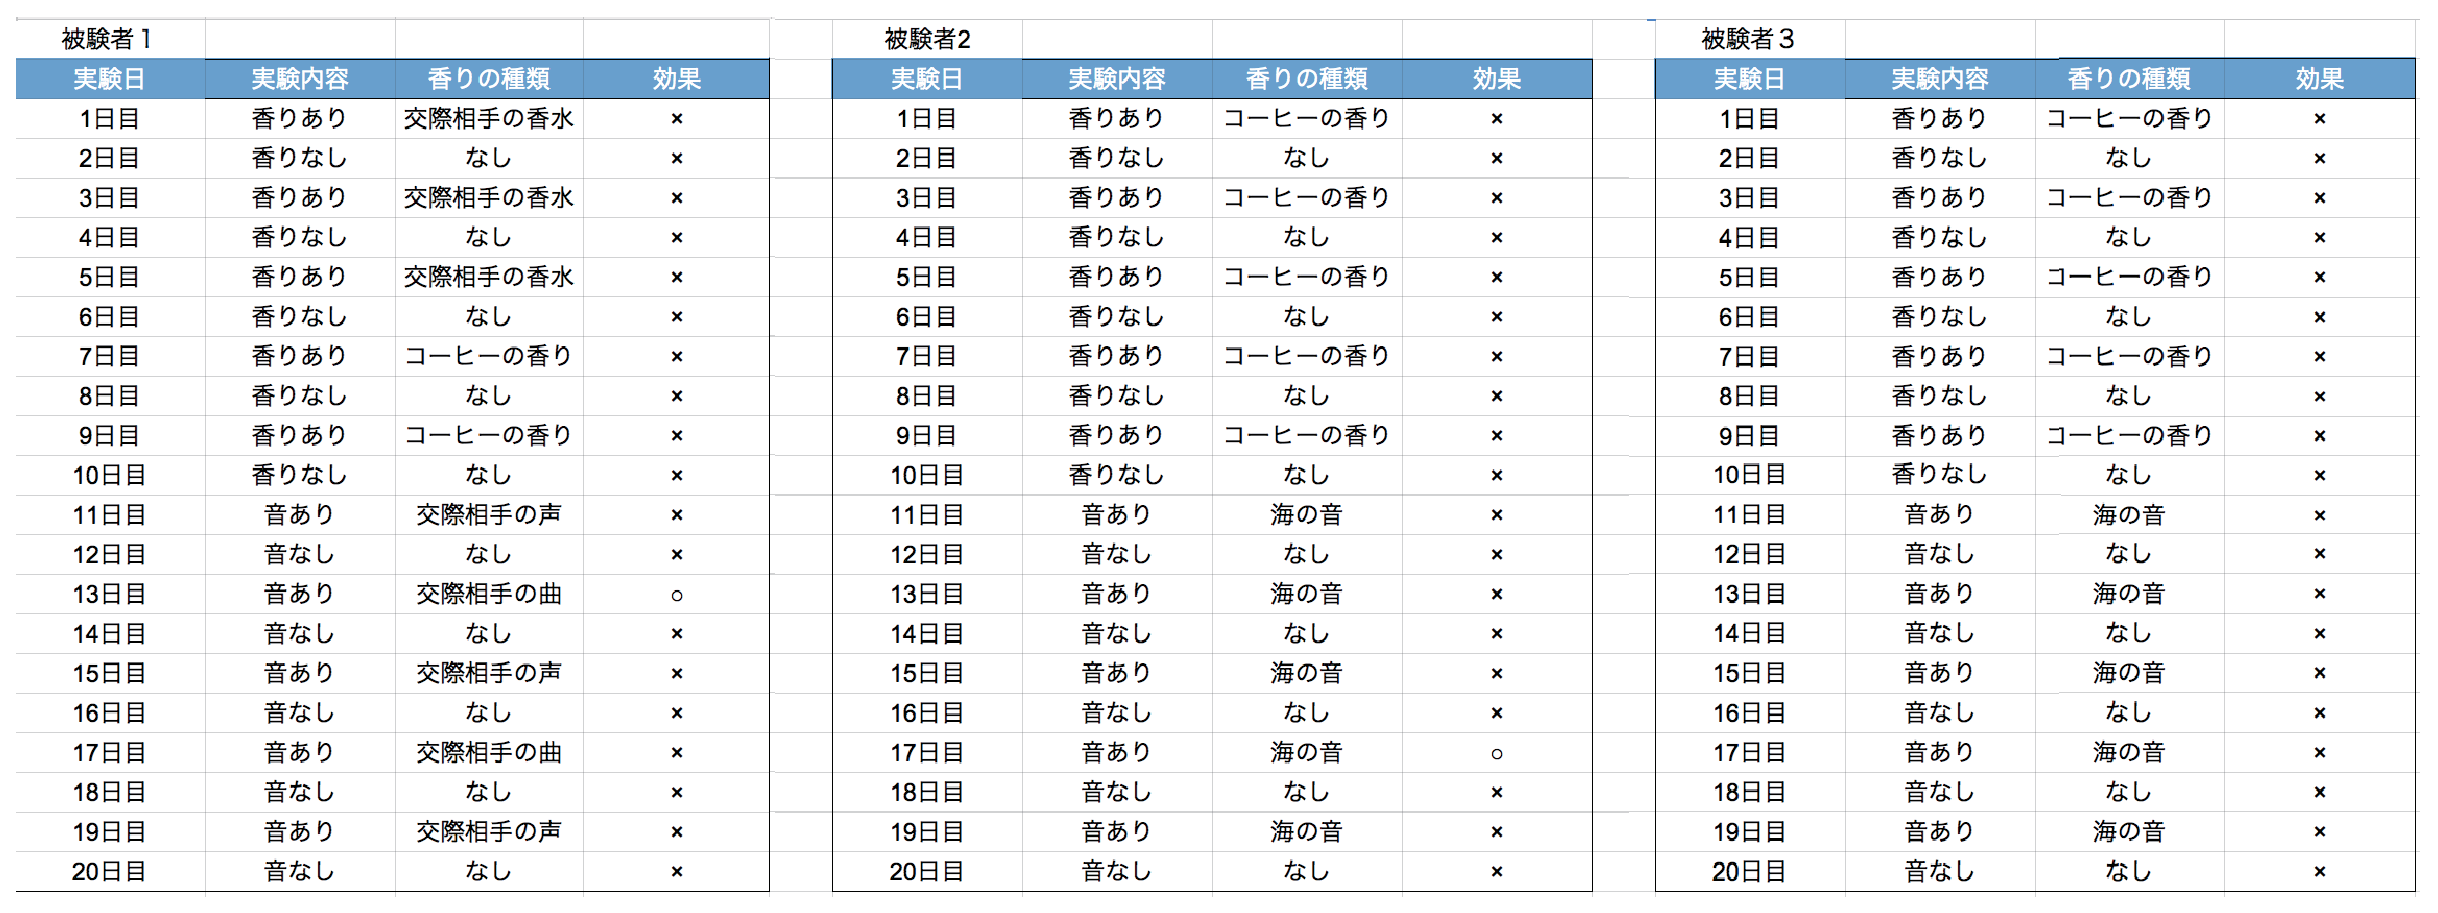
\includegraphics[width=15cm]{eps/smellExperiment.eps}
\caption{香りによる刺激の実験結果}
\label{smellExperiment}
\end{center}
\end{figure}

\subsection{睡眠観測のプロトタイピング}
ユーザの睡眠深度のモニタリング方法はいくつかある。それぞれの方法をユーザビリティと機能性の2つの観点から、実験を通して分析する。

\subsubsection{脳波センサーによる観測}
 このプロトタイプではNeuroSkyのThinkGear ASICモジュールという脳波センサーを使用した。Theta波が4〜7.2HzかつDelta波が0.5〜4Hzである時をレム睡眠中であるとし自らが実験台となり装着して寝てみた。しかしこの手法は頭を締め付けられる感覚があり、且つ汗をかいてしまうのでユーザに負担がかかる。寝心地を損ねてしまうということがわかりセンサーの体と離す別の方法を試すことにした。
\begin{figure}[htbp]
\begin{center}
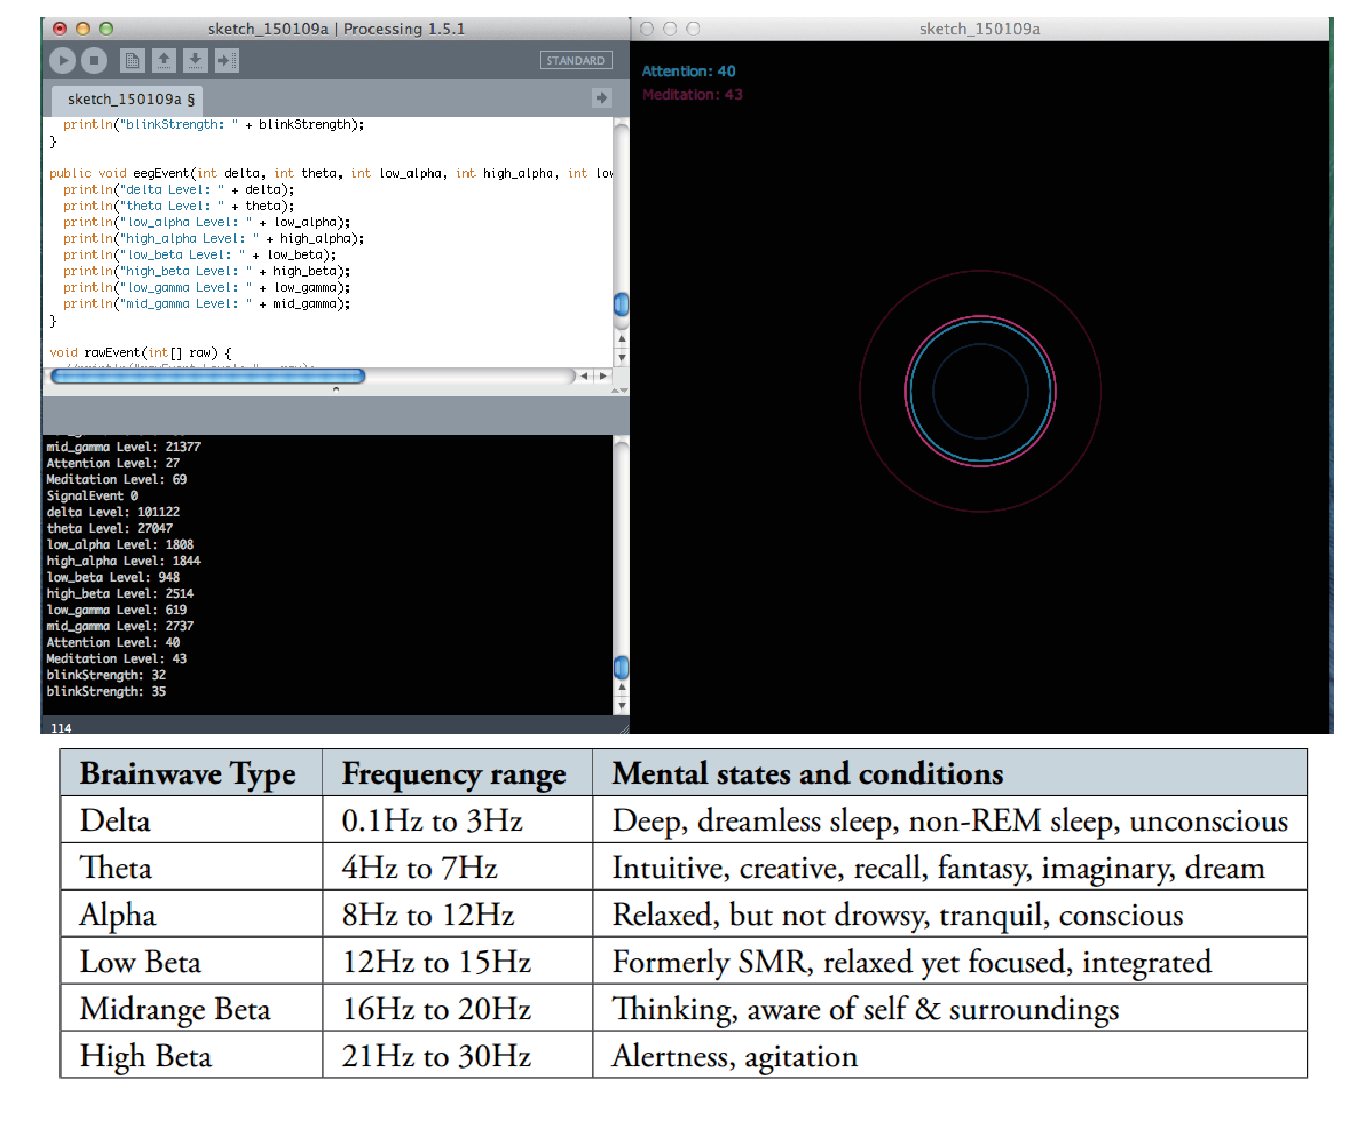
\includegraphics[width=10cm]{eps/brainWave.eps}
\caption{脳波センサーによるセンシングのプログラムと睡眠ステージと脳波の数値}
\label{brainWave}
\end{center}
\end{figure}

\subsubsection{心拍センサーによる観測}
 次に市販で売られている心拍センサーを追懐睡眠中の心拍数を観測することでレム睡眠を検出できるかどうかの実験をした。しかし寝ているときに指にセンサーを装着するのは発汗のを引き起こし、ユーザ体験の視点から非常に好ましくないということがわかりまたしても別の方法を試すことにした。

\begin{figure}[htbp]
\begin{center}
\includegraphics[width=10cm]{eps/heart.eps}
\caption{心拍センサーによるセンシング}
\label{heart}
\end{center}
\end{figure}

\subsubsection{kinectによる観測}
 このプロトタイプはKinectを使用して、ユーザの寝返りを検知して音楽を流すシステムである。図\ref{kinect}のようにkinectを天井に設置する。ウェラブルセンサーではないためユーザには負担がかからない。但し布団をかぶってしまうとkinectによる骨格トラッキングは難しい。そのためOpenCVのライブラリを利用して、画像処理を行った。\\
 寝返り判定の正確性を確かめるために、実際にベッドの上で寝返りを打ったとき音が鳴るかを試したところ、開発したプログラミングではノイズが多く出て誤作動が起きてしまうのでkinectを使うのは適切ではないと判断した。しかしプログラミングの能力が高い人により開発されれば、kinectによるトラッキングの精度もあげられるはずである。ただし、デバイス自体の価格が高いのと、取り付けに労力が必要とされることと、ポータブルではないため旅先では使えないという点で、本研究では好ましくないとした。

\begin{figure}[htbp]
\begin{center}
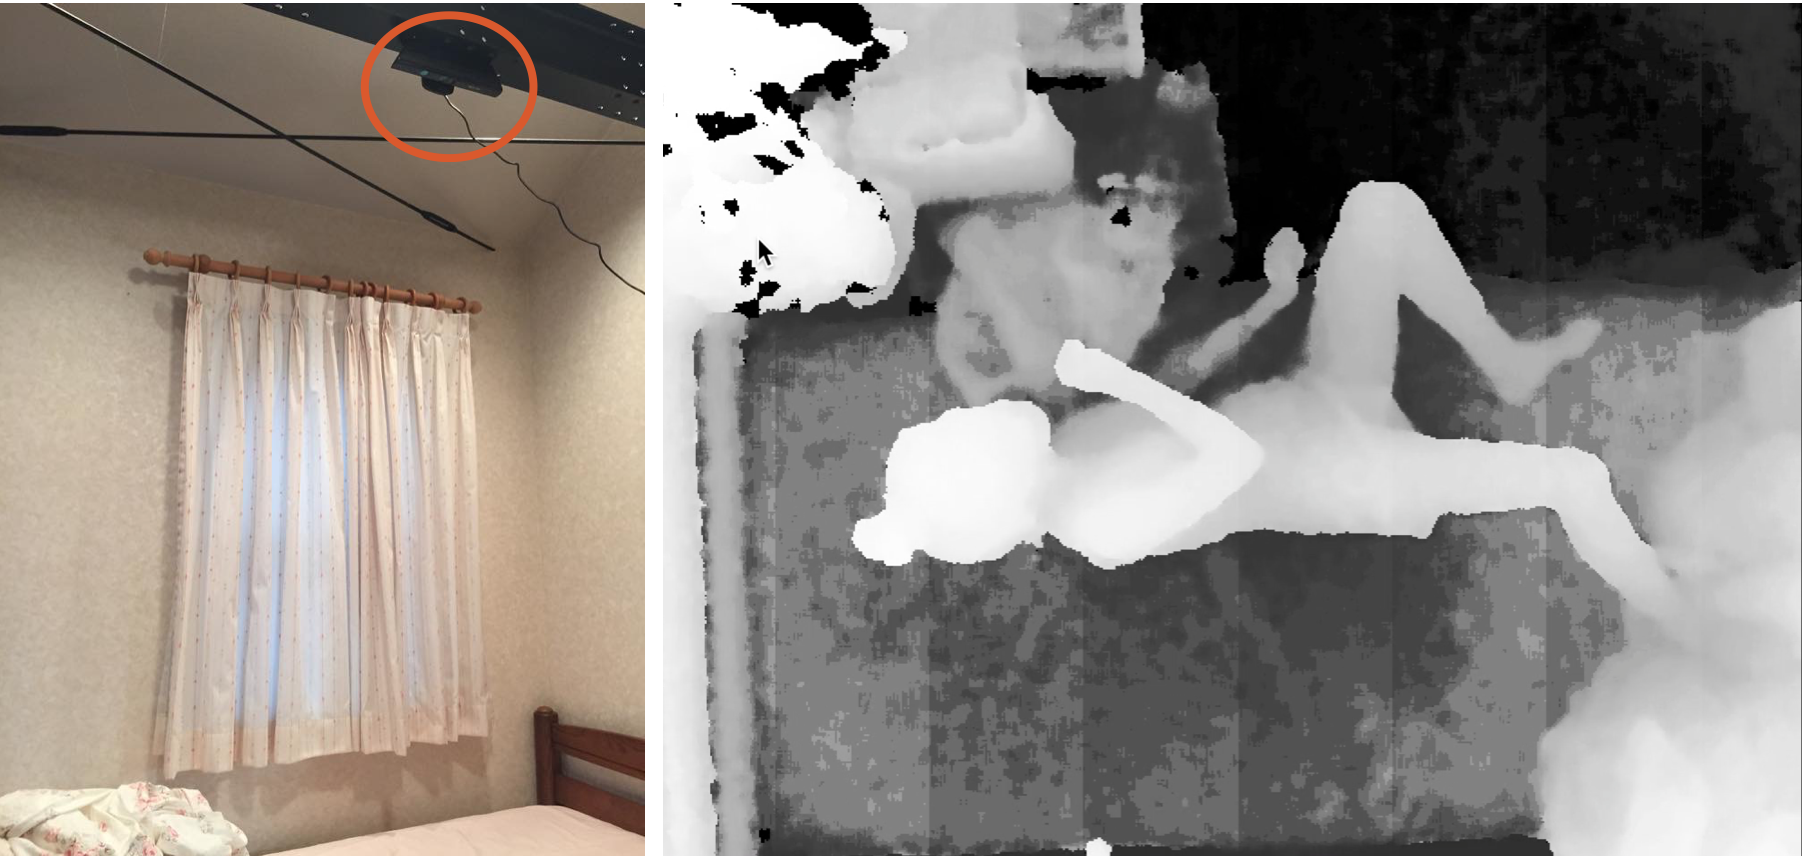
\includegraphics[width=15cm]{eps/kinect.eps}
\caption{kinectによるセンシング}
\label{kinect}
\end{center}
\end{figure}

\subsubsection{スマートフォンの加速度センサによる観測}
 最終的に多くの人々が既に使用していて、ユーザビリティーの視点から見てもっとも負担のかからないスマートフォンアプリケーションによるセンシングに試みた。スマートフォンで計測すときはウェラブルではないため身軽であるし、持ち運びが簡単なので旅中も使える。スマートフォンアプリケーションによるセンシング方法とその正確性については5章で述べる。

